\documentclass[12pt, letterpaper]{article}
\usepackage[utf8]{inputenc}
\usepackage{hyperref}
\usepackage{xcolor}
\usepackage{amsmath}
\usepackage{xfrac}
\usepackage{graphicx}

% \setlength{\parindent}{0cm}
% \setlength{\parskip}{1ex plus 0.5ex minus 0.2ex}
\newcommand{\hsp}{\hspace{20pt}}
\newcommand{\HRule}{\rule{\linewidth}{0.5mm}}


\newcommand{\com}[1]{{\small {\fontfamily{ptm} \selectfont \textcolor{red}{#1}}}}

\begin{document}


\begin{titlepage}
  \begin{sffamily}
  \begin{center}
  
  \begin{figure}
\centering
\begin{minipage}{.5\textwidth}
  \centering
  
\includegraphics[scale=0.27]{imt_mines_ales.jpg}
\end{minipage}%
\begin{minipage}{.5\textwidth}

  \centering
  
\includegraphics[scale=0.15]{fau-logo.png}
\end{minipage}
\end{figure}

    \textsc{\LARGE Ales School of Engineering}\\[2cm]

    \textsc{\Large third year internship report}\\[1.5cm]

    % Title
    \HRule \\[0.4cm]
    { \huge \bfseries Data-driven COVID-19 modeling\\[0.4cm] }

    \HRule \\[4cm]
    % \includegraphics[scale=0.12]{1_q21J8w3s_pUBQ8aiDFq7Pg.png}

    % Author and supervisor
    \begin{minipage}{0.4\textwidth}
      \begin{flushleft} \small
        Cyprien \textsc{Neverov}\\
        3A, 168\\ 
        Final Year Internship
      \end{flushleft}
    \end{minipage}
    \begin{minipage}{0.4\textwidth}
      \begin{flushright} \small
Chair in Applied Analysis, Department of Mathematics,\\
Friedrich-Alexander University\\
Cauerstr. 11, 91058 Erlangen, Germany\\
        \emph{Tutor:} Enrique \textsc{Zuazua}\\
      \end{flushright}
    \end{minipage}

    \vfill
    \vfill

    % Bottom of the page
    {\small March 9\textsuperscript{th} 2020 — July 3\textsuperscript{rd} 2020}

  \end{center}
  \end{sffamily}
\end{titlepage}

\begin{abstract}
\normalsize

\textsc{english -} The COVID-19 pandemic has challenged the way our modern societies work, consequently the study of this disease is of major interest. 
In order to have a better understanding of the evolution of the disease and provide insights on the future evolution, epidemiologists use mathematical modeling.
In this work, we attempt to apply system identification techniques to COVID-19-related data.
The goal is to explore what dynamics can be observed in the evolution of the number of cases and how it relates to the government control measures as well as its relation to social characteristics of the different countries.
One of the deliberate limitations of this analysis is the choice of purely data-driven models with very little a priori.
We observe that the system identification algorithms we use are prone to overfitting and that the problems we envisioned are hard to solve because we do not have the complete evolution of the pandemic yet.




\textsc{french -} La pandémie du COVID-19 remet en question le fonctionnement de nos sociétés et son étude est un enjeu majeur. 
Dans le but d'avoir une meilleure compréhension de l'évolution de la maladie ainsi que de donner des informations sur sa future évolution, les épidémiologistes utilisent les modèles mathématiques.
Dans ce rapport, nous exposons notre tentative d'utilisation des outils d'identifications de systèmes dans le contexte du COVID-19.
Le but est d'explorer les dynamiques de l'évolution de nombre de cas ainsi que de la lier aux mesures de contrôle prises par les gouvernements et les caractéristiques sociales des différents pays.
Une des limitations intentionnelles de cette étude est l'utilisation de méthodes purement basées sur les données avec très peu d'a priori.
Nous observons que les algorithmes d'identification de systèmes que nous utilisons ont tendance à faire du overfitting ainsi que les problèmes que nous avons choisi sont difficiles à traiter avec l'information encore incomplète de la pandémie.



\end{abstract}

\newpage
\tableofcontents


\section{Introduction}
Since its outbreak in late 2019 in Wuhan, China the COVID-19 virus has spread all over the world and has challenged the social and health systems of many countries. 
The pandemic has also triggered a huge interest from all disciplines of science and countless researchers have contributed to the better understanding of the characteristics of this novel disease. 
An astonishing number of more than 64.438\footnote{Website accessed on the 29\textsuperscript{th} of August 2020.} COVID-19 related contributions is available on the \href{https://search.bvsalud.org/global-literature-on-novel-coronavirus-2019-ncov/}{WHO website} and all of these articles where published after the first of January 2020.

Those contributions cover an extremely wide range of aspects of the pandemic: from the behavior of the virus on a microscopic level and it's lifespan on different surfaces to the impact of the lockdown on the psychology of the population. 
One very important aspect of the pandemic is obviously the understanding of it's evolutions and consequently it's modeling and forecasting. 
Modeling is very important because it is the only way for decision-makers to implement the right policies at the right time. 
A good predictive model can help to choose what kind of measures to implement, like school closing or travel ban and also when to stop these measures.

The goal of this work is to explore the usage of a data-driven system identification tool for COVID-related data. 
The most common way of modeling a disease is through compartmental models. 
They divide the population into different compartments like susceptible (not yet infected by the disease), exposed (infected but not yet infectious), infected, recovered. 
The interaction processes between the different compartments are governed by a set of simple ODEs. 
This framework was introduced almost a century ago and is flexible enough to model most of the effects and controls of the disease and allows for arbitrarily complex models. 
The classic epidemiological approaches will be further introduced in section \ref{sec:sir}.

In this work we deliberately choose to not base our modeling on these classic techniques and concentrate on the identification of dynamic processes in the evolution of the disease with very little a priori.
The different approaches considered in this work all gravitate around an algorithm proposed in \cite{sindy} called {\em system identification of nonlinear dynamics}. 
The details about this methodology will be explained in section \ref{sec:sindy}. 
In a few words, this algorithm allows to identify the dynamics from observed data through a sparse regression and based on a user-defined library of candidate functions. 
Throughout this work, we will use this algorithm in combination with datasets collected from different sources in order to better understand both the dynamics of the pandemic and the specificities as well as the limits of this algorithm. 

The ability to identify the dynamics from data is a fundamental challenge. 
Even though the centuries of research have given a good understanding of surrounding physical and natural phenomena, there are plenty of more complex systems that are yet to be modeled. 
Examples of such systems might be the patterns in weather and climate, epidemiology, power grids, etc. \cite{sindy}. 
The present work is an attempt at applying such a dynamics identification tool on real world data. 
However, it is important to highlight that, as mentioned earlier, the field we are targeting (epidemiology) already has some very powerful modeling frameworks. 
In this context it is very hard to achieve interesting results in terms of modeling.

The rest of this report is constructed as follows: in section \ref{sec:sir} we present the classic and already existing modeling approaches for epidemiology. In section \ref{sec:sindy} we thoroughly describe the system identification algorithm on which this work is based. Then in section \ref{sec:data} we present and discuss about the data that we use in our modeling. In the next section \ref{sec:modeling} we talk about the different modeling approaches that we envisioned for this work and describe the results. After this, in section \ref{sec:discussions} we comment on the results and try to give some elements about the reasons our methods are challenging to use. Finally we sum-up our conclusions in section \ref{sec:conclusion}.

\section{Classic epidemiological modeling techniques}\label{sec:sir}

\subsection{SIR models}

The most basic model of this kind is the SIR model that tracks the number of susceptible, infected and recovered people in the sample. 
It was originally proposed in \cite{sir} and has become the most widely used epidemiological model.
This very simple model is formulated by the following set of equations:

\begin{equation}\label{eq:sir}\
\begin{split}
\dot{S} = &- \beta SI \\
\dot{I} = &\beta SI - \gamma I \\
\dot{R} = & \gamma I
\end{split}
\end{equation}
where $\beta$ and $\gamma$ are the parameters of the disease. 
$\sfrac{1}{\gamma}$ is the time a person remains infectious while $\beta$ quantifies the infectiousness of the disease. 
The ratio $\sfrac{\beta}{\gamma}$ is usually denoted $R_0$ and called the basic reproduction value. 
It is a very important characteristic of the disease because it represents the average number of people a single person is susceptible to infect. 
All the measures introduced by the governments in order to limit the impact of the disease were targeted at reducing this $R_0$ value. 

These models can be further elaborated in several ways. 
The first sophistication can be introduced by adding additional compartments like {\em exposed, quarantined, hospitalized, deceased} to further mimic the real interactions between these different categories of the population. 
It is clear that COVID-19 has a lot of delay in it's dynamics \cite{delay} because it can have an incubation time of up to two weeks. 

In order to take this into account it might be necessary to add at least an "exposed" compartment. 
Thus, when infected, a person is not immediately infectious and must stay a few days in the "exposed" compartment. 
A few examples of more sophisticated SIR models and adapted specifically to COVID-19 can be seen in \cite{seir, seir2} but as mentioned earlier there is a huge number of such adaptations.


Secondly, knowing that the different age groups of the population are affected in very different ways by the disease, it might be interesting to subdivide the population into the relevant age groups in order to have a more precise control over the parameters. 
For example the mortality rate is almost equal to 0 for children and is very high for the people above 80 years of age. 
Age subdivision is also a widely used practice and can be seen in \cite{age-groups, spatial2} for example.

Thirdly, one very classic way of making the models more complex and precise is by subdividing the region of interest into smaller sub-regions and to have a state for each of these sub-regions. 
For example a country can be sub-divided into regions or counties. 
Some parameters traducing the migrations between these regions can be introduced. 
One can imagine that this kind of modeling can be very useful for policy-makers to adopt more precise and local measures. 
Few examples of such models can be found in \cite{spatial, spatial2}. 
These models are usually called {\em spatial SIRs}. 

Finally, there is no limitation to the complexity of the models that can be built on the basis of the SIR models. 
They can be combined and adapted to a very wide range of problems. 
An example of such use might include adding the relevant compartments to model the usage of a tracking mobile app that facilitates the isolation of people who have interacted with another infected person \cite{mobile-app}.

\subsection{Other modeling techniques}

The modeling of infectious diseases is however not limited to the aforementioned compartmental models and lots of different approaches from different disciplines exist. 
Other approaches for modeling the spread of an infectious disease include:

\begin{itemize}

\item \textbf{Statistical models} are more inclined towards capturing the random nature of the infectious diseases. 
Thorough reviews of these approaches can be found in \cite{statistical, statistical2}.

\item \textbf{Gravity models} can be used as standalone models or in conjunction with the compartmental approach and are called "gravity" models because they rely on considering the effect of distance and the size of donor and recipient communities \cite{gravity, gravity2}. 

\item \textbf{Network-based models} are built on the assumption that the spread of human disease follows its specified contact or spreading paths such as transportation or social contact networks \cite{network-based, network-based2}.

\item \textbf{Agent-based models} are based on the belief that individuals and their mutual differences are the key to understanding the spread of an infection \cite{agent-based, agent-based2}.
\end{itemize}

Additionally, hybrid approaches combining different methods are considered in the literature \cite{hybrid, hybrid2} as well as more computationally-oriented methods like cellular automata \cite{automata}
A thorough review about the modeling of infectious diseases can be found in \cite{epidemic-modeling-review}.

\section{Sparse identification of nonlinear dynamics}\label{sec:sindy}

In this section the central algorithm used in this work will be introduced. 

\subsection{Algorithm}

This algorithm lies on the crossroads between dynamic modeling and machine learning. 
On one hand this algorithm is able to fit the observed data much like more classic machine learning algorithms would do. 
And on the other hand it does so by finding governing ODEs in observed data. 
In theory this allows to model an arbitrarily complex phenomenon while having the interpretability of a set of simple ODEs. 
We will see that in practice, when dealing with real-world data and complex problems this technique doesn't hold up to these expectations.

Machine learning is an extremely young branch of science as opposed to dynamic modeling, because mathematicians, physicists and engineers have been modeling physical phenomena for centuries. 
The shift that happened in the recent years is that (1) computational power has significantly increased and now allows for computations of unprecedented complexity and (2) observation data is getting increasingly available as sensor prices go down. 
The combination of these two tendencies opens new horizons for modeling increasingly complex processes.  


It was quickly mentioned in the introduction that this algorithm has two key features: (1) it relies on a user defined set of candidate functions and the result will only be as good as the candidate functions are with respect to the problem; (2) it uses sparse regression (some weights are gradually zeroed-out) in order to find the most parsimonious formula that still fits the data.

The whole methodology to discover the dynamics can be divided into 3 steps. 
Let's say that we have a series of observations $(\mathbf{x}(t_1), \mathbf{x}(t_2), \dots, \mathbf{x}(t_m))$ where $\mathbf{x}$ is the state or the vector state of the system of interest and $m$ is the number of observations. 
Our goal is to find a function $f$ such that:

\begin{equation}\label{eq:diff}
\dot{\mathbf{x}} = f(\mathbf{x})
\end{equation}



\begin{enumerate}
	\item It is more convenient to work with matrices to do the computations so our first step will be to divide the available data into two matrices:
	$$X = 
	\begin{bmatrix}
	\mathbf{x}(t_1) \\
	\mathbf{x}(t_2) \\
	\vdots \\
	\mathbf{x}(t_m)
	\end{bmatrix}
	\text{ and }
	\dot{X} =
	\begin{bmatrix}
	\dot{\mathbf{x}}(t_1) \\
	\dot{\mathbf{x}}(t_2) \\
	\vdots \\
	\dot{\mathbf{x}}(t_m)
	\end{bmatrix}
	$$
	here the dot notation denotes the time-derivative and it can be either directly observed or computed numerically.

	\item The second step of this algorithm is the augmentation of the state with the candidate functions. 
	Let's say that we have a set of $p$ candidate functions ($f_1, f_2, \dots, f_p$) that we want to use for this identification. 
	What we need to do is to construct a matrix $\theta(X)$:
	$$\theta(X) = 
	\begin{bmatrix}
	f_1(\mathbf{x}(t_1)) & f_2(\mathbf{x}(t_1)) & \cdots & f_p(\mathbf{x}(t_1))\\
	f_1(\mathbf{x}(t_2)) & f_2(\mathbf{x}(t_2)) & \cdots & f_p(\mathbf{x}(t_2))\\
	\vdots & \vdots  & \ddots & \vdots\\
	f_1(\mathbf{x}(t_m)) & f_2(\mathbf{x}(t_m)) & \cdots & f_p(\mathbf{x}(t_m))\\
	\end{bmatrix}
	$$

	\item Finally we can run the optimization and find the best set of $\xi_1, \xi_2, \dots, \xi_p$ that minimize the following equation in the least squares sense:
	$$\dot{X} = \theta(X) \times \Xi \text{ where } \Xi = 
	\begin{bmatrix}
	\xi_1 \\
	\xi_2 \\
	\vdots \\
	\xi_p
	\end{bmatrix}
	$$
	After the best $\xi_1, \xi_2, \dots, \xi_p$ were identified, the very small $\xi$ (those that have an absolute value under a certain threshold called {\em cutoff value}) can be removed from the equation alongside with the candidate function they correspond to. 
	And then the least squares minimization can be ran again with the new subset of candidate functions and weights. 
	After doing this thresholding a few times the algorithm converges.

\end{enumerate}

This is the very general definition of the algorithm, in our case we used almost exclusively polynomial terms of the state as candidate functions. 
For example if our state is $\mathbf{x} = (s, i, r)$ like in the compartmental models, then our candidate function be: 
$\mathbf{x} \mapsto 1,
\mathbf{x} \mapsto s,
\mathbf{x} \mapsto i,
\mathbf{x} \mapsto r,
\mathbf{x} \mapsto s^2,
\mathbf{x} \mapsto si,
\mathbf{x} \mapsto sr,
\dots,
\mathbf{x} \mapsto r^n$ where $n$ is the maximum degree of the polynomial terms that we consider. 
If the state of the system is $\mathbf{x} = x$ like if we just tracked the cumulative number of cases in a single country, then the candidate functions would be: $\mathbf{x} \mapsto 1,
\mathbf{x} \mapsto x,
\mathbf{x} \mapsto x^2,
\mathbf{x} \mapsto x^3,
\dots,
\mathbf{x} \mapsto x^n$. 
A more thorough discussion about polynomial terms is held in section \ref{sec:polynomials}.

Another remark is that this algorithm works equally well with an iterative formulation as it does with the differential one like in equation \ref{eq:diff}.
In the iterative case we would have a series of observations ($\mathbf{x}_1, \mathbf{x}_2, \dots, \mathbf{x}_m$) and the goal is still the same but we want $f$ to express the dynamics in an iterative way:

\begin{equation}\label{eq:it}
\mathbf{x}_{t+1} = f(\mathbf{x}_t)
\end{equation}

This is slightly more convenient because it prevents us from numerically computing a derivative which obviously introduces some errors. This is achieved by dividing the two matrices in the following way:


$$X = 
\begin{bmatrix}
\mathbf{x}_1 \\
\mathbf{x}_2 \\
\vdots \\
\mathbf{x}_{m-1}
\end{bmatrix}
\text{ and }
X_2 =
\begin{bmatrix}
\mathbf{x}_2 \\
\mathbf{x}_3 \\
\vdots \\
\mathbf{x}_m
\end{bmatrix}
$$
and minimizing $X_2 = \theta(X) \times \Xi$ instead.

One can notice that this algorithm is very simple and sound quite intuitive.
This work was further extended in a second paper \cite{sindy2} that is more centered on PDE identification instead of working with ODEs. 

\subsection{Hyper-parameters}

If we consider this algorithm as a machine learning methodology then its hyper-parameters would be:
\begin{enumerate} 
    \item the choice of the set of candidate functions;
    \item the cutoff value; 
\end{enumerate}
and both these parameters deserve a discussion.

\subsubsection{Cutoff value}

We previously mentioned that the cutoff value is the parameter used for thresholding the small weights in the learning process. 
In fact, this parameter allows us to choose the sparsity of the resulting model and thus choose the required balance between accuracy and complexity of the model.

In practice, due to the low computational cost of this algorithm\footnote{20.2 ms ± 359 µs for 100 data points and 10 candidate functions on our i7 machine.} we are able to compute the results for a very wide range of cutoff values and to choose the one that we prefer. 
Usually the one satisfying the philosophy of "Ockham's razor", in other words the highest cutoff value that has satisfying fitting of the data. 
An example of such a plot can be seen on figure \ref{fig:tradeoff}. 


\begin{figure}[h]
\centering
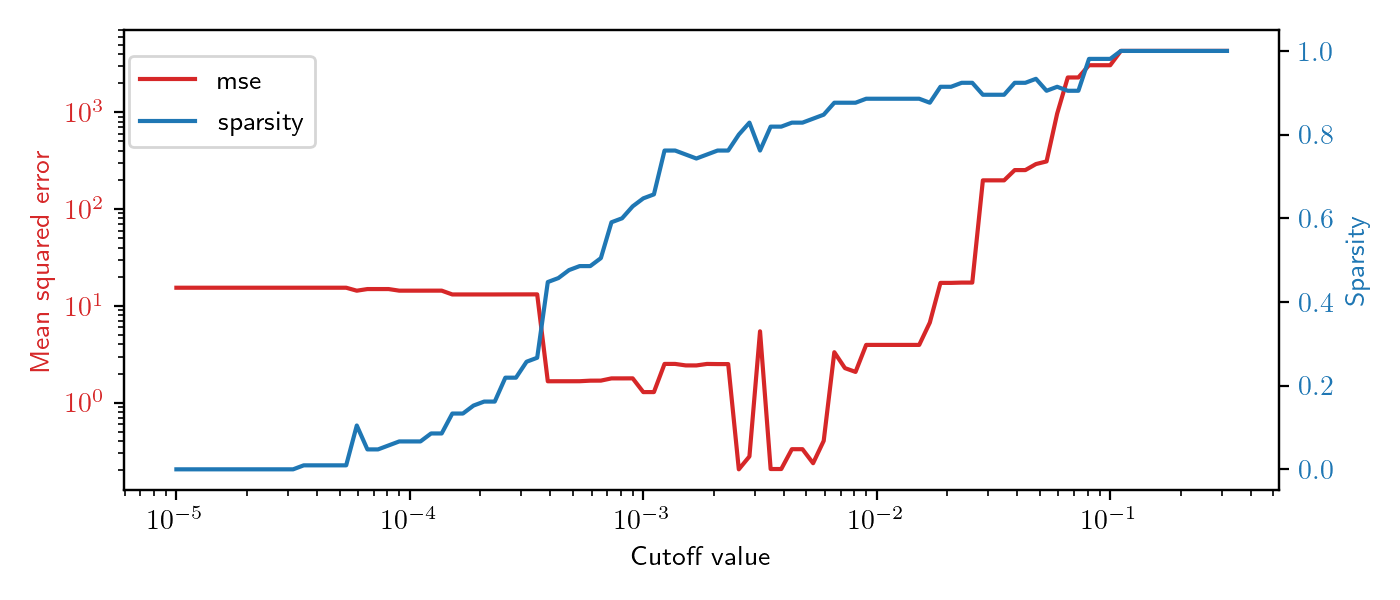
\includegraphics[scale=0.8]{tradeoff.png}
\caption{Illustration of the bias-variance trade-off for the system identification algorithm.}
\label{fig:tradeoff}
\end{figure}

This plot depicts the evolution of the mean squared error and the sparsity with respect to the cutoff value.
The cutoff value ranges from $10^{-5}$ to $10^{-0.5}$, this was manually selected so that the sparsity ranges from 0 (all coefficients are non-zero) to 1 (all coefficients are zero).
This graph was generated using synthetic data\footnote{Data includes 300 observations and polynomials of a maximum degree of 4 were used as candidate functions.} from a \href{https://en.wikipedia.org/wiki/Lorenz_system}{Lorenz attractor}, because it illustrates the best-case scenario where the actual dynamics are included in the candidate functions and there is nothing preventing the algorithm from converging to the actual formulation.
One can notice that there is a minima in the mean squared error around $4 \times 10^{-3}$. In the same region the sparsity reaches 0.8 which means that the best model has less than 20\% of active coefficients.

In the problems that we treated in this work, when the real dynamics do not appear in the candidate functions (because they are too complex) the mean squared error curve doesn't have the minima in the middle but rather the most complex system is the most accurate. 
In this case a plot of this kind can help to choose how much accuracy are should we sacrifice to gain sparsity.

Sometimes it can be very relevant to plot both the training and test error in order to have a better idea about how the model generalizes.




\subsubsection{Candidate functions}\label{sec:polynomials}

In a simple problem, we just want our candidate function to include the real dynamics. 
The authors mostly use polynomial terms as candidate functions because the dynamics they identify in the examples are actually polynomial terms of the variables of the state. 
In the 7 examples of identification that they provide, the candidate functions always include the real dynamics. 

In more general cases and more complex problems, we cannot guarantee the same thing. 
And instead we use polynomials as approximators and hope that they will be expressive enough to capture the evolution. 
Obviously, it is very important to make this distinction between making a library large enough to include the real dynamics and using polynomials as universal approximators. 

Our choice of polynomial basis functions was motivated by the fact that the authors propose their usage, that they are quite simple to use and understand and finally that the study of basis functions is not completely in the scope of this work. 
Consequently, the question of whether they are the more relevant candidate functions in our case remains not fully answered. 
Indeed an elaboration was explored by using rational functions instead of polynomials. 
The full discussion is available in appendix \ref{app:rational}.
Our main conclusion from this superficial experiment was that with similar maximum degrees, rational functions provided little to no advantage over the polynomial ones in terms of mean squared deviation while requiring a less-convenient non-linear least squares fitting.



\section{Data}\label{sec:data}

Data plays a crucial role in our approach because our aim is to base all the modeling on the observation data.
In this section we will describe what kind of data we used for our modeling.

\subsection{Observing the pandemic}\label{sec:jhu}

Because this pandemic has no precedents, the metrics people used to track the state of the disease have evolved during the course of the disease. 
For example, on the February 13th 2020 the redefinition of what a "case of infection" is according to the WHO led to a huge spike in new cases in China. 
This example highlights the fact that the observation data in not completely reliable. 
Furthermore, due to the big differences in healthcare systems in different countries as well as on a regional scale, it can be unfair to compare the numbers. 
An example of such difference might be the testing policy. 
Indeed countries around the word have implemented vastly different testing approaches, from very selective testing of only symptomatic people to massive testing like in Germany and Korea. 
This difference in the number of tests leads to a big difference in the test positivity rate. The higher the test positivity rate the less we are confident about our real understanding of the scale of the epidemic.

In our study, we mainly used the {\em cumulative number of cases}. 
Basically, it is the total sum of people that got infected in a given region, its evolution usually looks like a logistic function. 
Not to be confused with the "I" in an SIR model which accounts for the number of currently infected people. 
Tracking the evolution of the pandemic through the cumulative number of people is convenient because (1) it is the minimum information we need to have an idea about the state of the disease in the population and (2) even if the quality of the data is not perfect it is the most widely available information (for example, the number of recovered people is missing or is not reliable for a big number of countries).

The most widely used resource for tracking the number of cases worldwide is the repository of the John Hopkins University. They have collected the numbers from all over the world and provided required APIs for all researchers and visualization dashboards to use. They also provide information about recovered cases but as mentioned earlier, the quality of the data is undermined by lots of discontinuous update spikes.

A quick visualization of this dataset of 188 countries can be seen in figure \ref{fig:all_trajectories}. 
For example, the coloration per continent shows how first the pandemic touched Asia and a month later arrived to Europe. 
It is also noticeable how Africa was the last continent to be affected.
More generally, we can see that all trajectories have a somewhat similar evolution.

\begin{figure}[h]
\centering
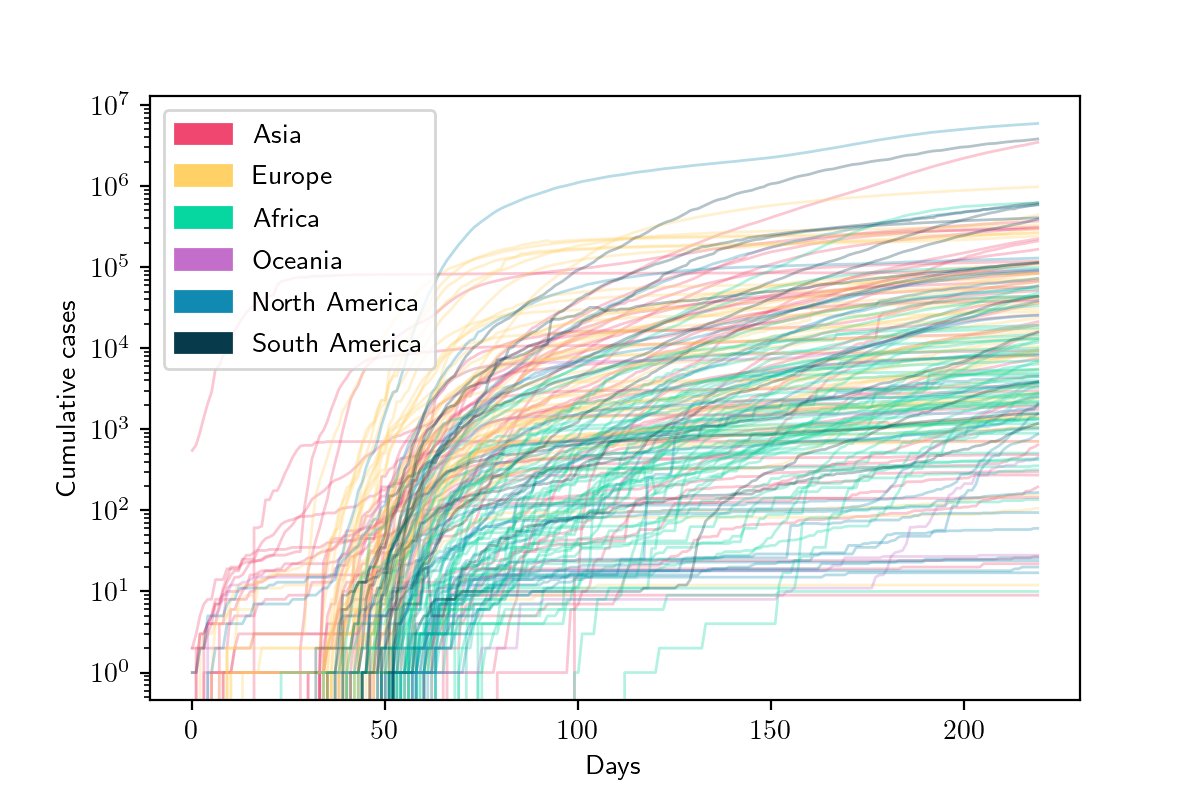
\includegraphics[scale=0.8]{all_trajectories.png}
\caption{All trajectories of the cumulative cases in all 188 countries.}
\label{fig:all_trajectories}
\end{figure}

\subsection{Observing the government measures}\label{sec:stringency}

In our modeling approach we also need to take into account the measures that were taken by the governments to prevent further spreading of the disease like school closing, travel ban, work from home recommendations and alike. 
For this we relied on the information gathered by a group of researchers from Oxford \cite{stringency}. 
They tracked the measures that were implemented in most of the countries worldwide and provided a convenient way to retrieve this information as indicators and also they compiled all of this information into a "stringency" index. 
This index is a linear combination of all the indicators that they observed and it's meant to evaluate how strict are the measures implemented by the governments but it has no information about their effectiveness or performance. An example of a stringency index can be seen on figure \ref{fig:france_stringency}

\begin{figure}[h]
\centering
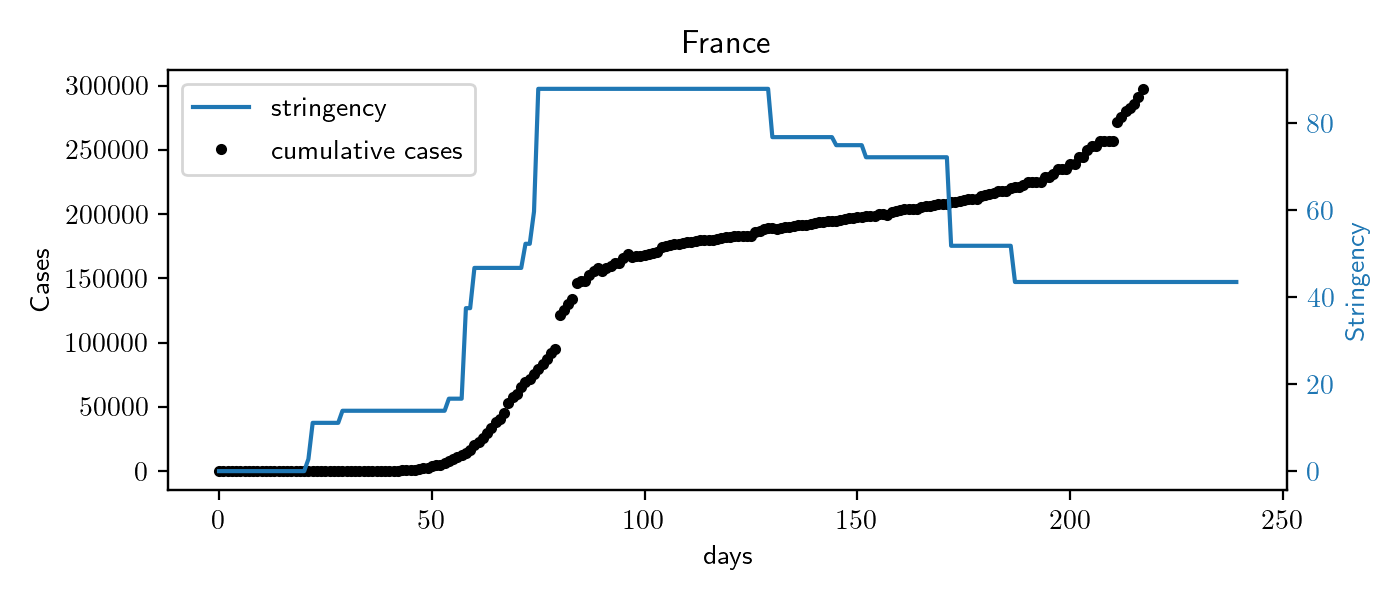
\includegraphics[scale=0.8]{france_stringency.png}
\caption{Example of stringency index.}
\label{fig:france_stringency}
\end{figure}

\subsection{Other information}\label{sec:worldbank}

Since the adopted methodology of this work heavily relies on the principles of machine learning and data science, we included additional datasets into our modeling because usually, the more relevant information we have, the better the results. 
For example, in one of our experiments we chose to make a model that would take into account the trajectories of all available countries (more about this in section \ref{sec:global}). 
In order to inform the model about the present country, we added more than 40 indicators relevant for the pandemic about the country (health, hygiene and demographic descriptors). 
A few examples of those descriptors can be: the human development index, the total population, the number of hospital beds per 1000 people, the number of people of 65 years and above, percentage of people using at least basic sanitation services, percentage of death caused by injury and so on.
This information was available to us through the World Bank API \cite{indicators}.

\section{Modeling}\label{sec:modeling}

In this section we will introduce the different experiments that we did with the tools and data that we described earlier. Three experiments will be described in depth and the rest will have a more concise presentation.

\subsection{Cumulative number of cases and forecasting}

The most obvious and easy way of using the system identification algorithm with COVID-19 data is to model the number of cumulative cases in a single country. If we define $\mathbf{x}_t$ as the number of cases in the country of interest at day $t$. Then, we want to find a function $f$ so that:
$$\mathbf{x}_{t+1} = f(\mathbf{x}_t)$$

When using polynomial terms as candidate functions we would look for a purely polynomial formulation of the dynamics because there is only one variable in the state. 
Which can be mathematically written as:
$$\mathbf{x}_{t+1} = \sum_{k=0}^p \xi_k \mathbf{x}_t^k$$
where $p$ is the maximum degree of the polynomial terms.

For example we can apply this method to the evolution of the cumulative number of cases in Germany an this is the formula we will end-up with:
$$\mathbf{x}_{t+1} = 1.24 \cdot \mathbf{x}_t - 0.9 \cdot \mathbf{x}_t^2 + 1.13 \cdot \mathbf{x}_t^3 - 0.47 \cdot \mathbf{x}_t^4$$
assuming a maximum degree of 4 and that $\mathbf{x}_{t}$ is the number of cumulative cases multiplied by $3 \cdot 10^{-5}$. 
The figure \ref{fig:germany} represents the trajectory of the real data as well as the trajectory of the identified model. 
One can see that this model fits fairly well the observation data and that the extrapolation looks fairly plausible. 
% Identified models in all countries are available in appendix \ref{app:all-countries}.


\begin{figure}[h]
\centering
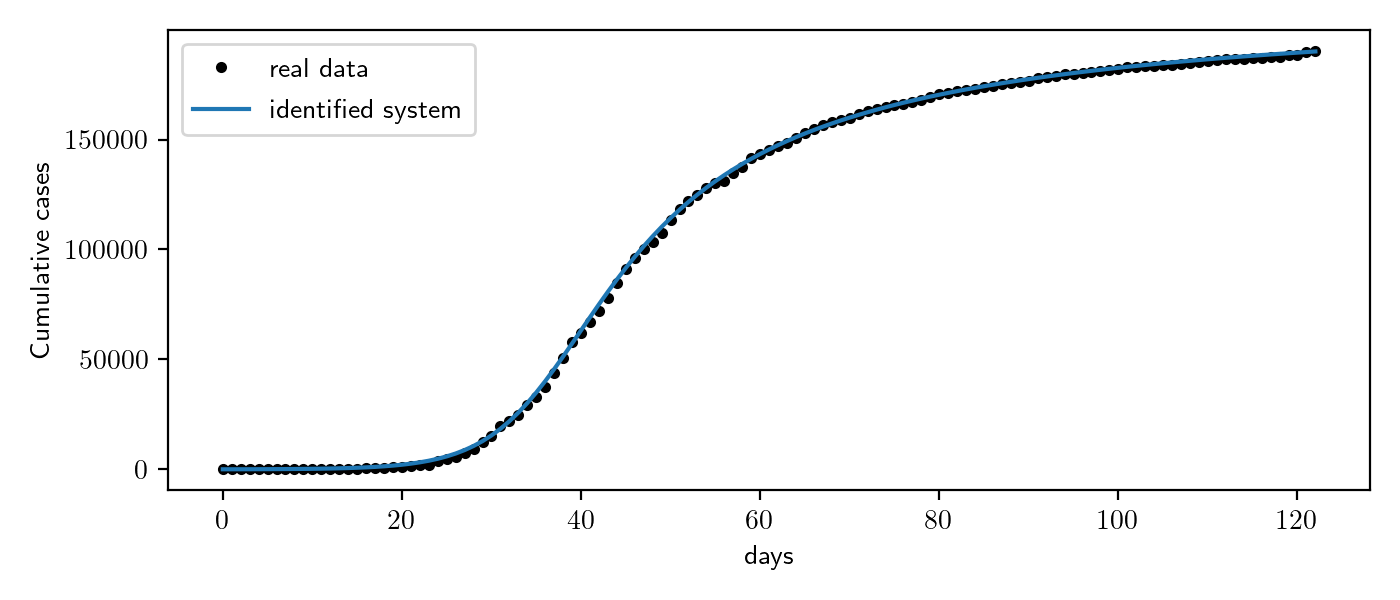
\includegraphics[scale=0.78]{germany.png}
\caption{Example of fitting the simple trajectory of cumulative cases for Germany.}
\label{fig:germany}
\end{figure}

Given that the identified model is extremely simple and has only one variable we cannot retrieve much useful information from it apart from the extrapolation of the number of cases in the next few days. 
For this reason, the main application of these country-wise models is forecasting. 
In order to have a better idea of how these very simple identified models compare to more advanced forecasting techniques we compared them to an auto-regressive integrated moving average (ARIMA) statistical model. We chose this particular model because there are examples of authors using it for COVID forecasting \cite{arima, arima2}.

The experiment was build as follows: we identified the dynamics of the cumulative number of cases in 118 countries with maximum degrees of the polynomials ranging from 2 to 7. 
We kept the last two weeks of available data out of the training set in order to evaluate and compare the models on a one and two weeks forecast horizon.
We trained an ARIMA$(1, 2, 1)$ model on the same training data in each of the countries and then we compared the results. 
The trajectories in all countries were rescaled so that the last value of the time-series is 1. 
This allows the models to more easily learn the parameters and to be able to fairly aggregate the mean squared deviation to do quantitative comparisons.

\paragraph{Results} The forecasts of the ARIMA model are fairly similar in terms of mean squared error to the result of the best performing identified system (the one that has the maximum degree that performs best on a given country). 
In terms of frequency of best results, the ARIMA model seems to have better results (in 55\% of the countries ARIMA has the best forecast for both forecast horizons). 
Figure \ref{fig:forecast_frequency} shows the different percentages of best predictions.
In terms of errors both methods are also quite similar but the ARIMA model is still slightly better that the dynamic models. 
% A more thorough description of the results of this experiment is available in appendix \ref{app:forecast}.

One interesting point to highlight is that there is no set of candidate functions that performs consistently better than the others. 
The wide range of maximum degrees that we chose for the experiment shows that more complex models (with higher maximum degree) do not necessarily perform better than the simpler ones.
In fact, this inconsistency is disadvantageous because if we were to make a real forecast we would have a hard time deciding what maximum degree to trust more. 


\begin{figure}[h]
\centering
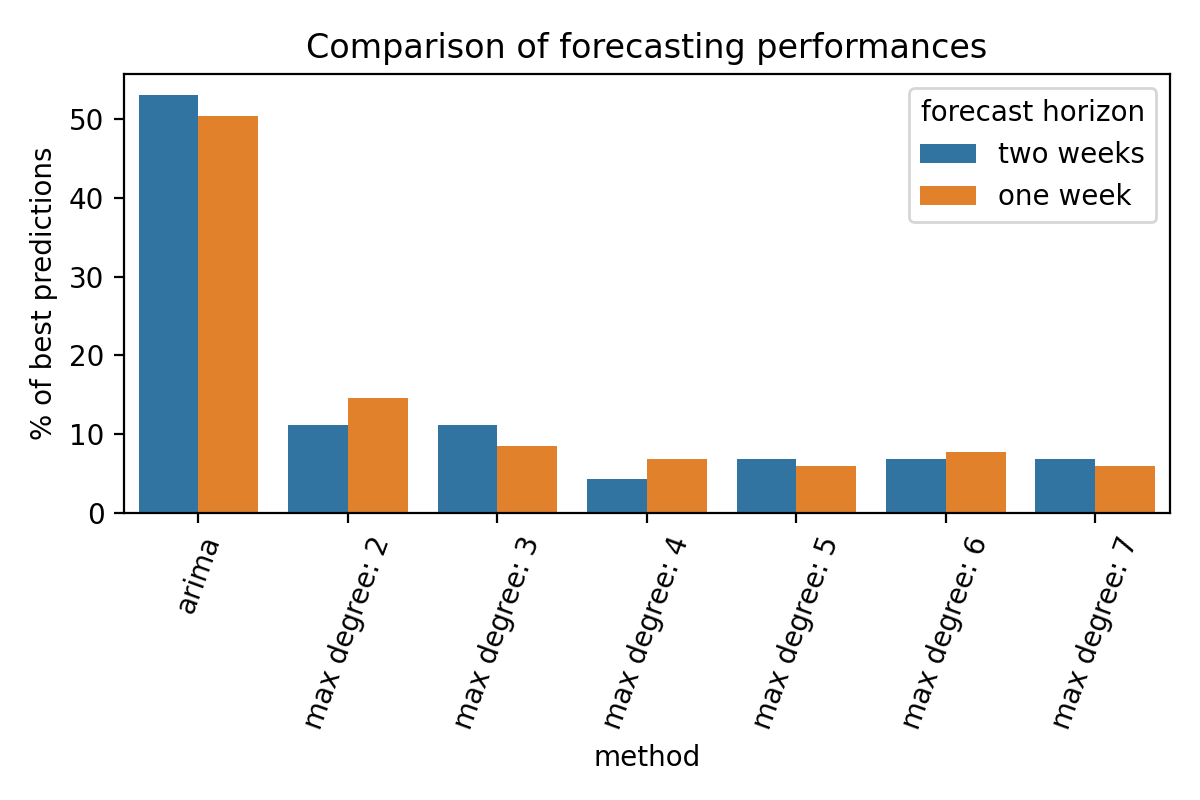
\includegraphics[scale=0.8]{forecasting.png}
\caption{Results of the SINDy vs. ARIMA experiment in terms of the percentage of countries with the best forecast.}
\label{fig:forecast_frequency}
\end{figure}

\paragraph{Limits of the experiment}

The ARIMA forecasting model requires that the time-series verifies some assumptions like stationarity and that there are no other predictors. 
The statistical model is also not very easy to parametrize and requires the data to be preprocessed for better results.
Given that we have done the bare minimum of these manipulations it would not be fair to quantitatively compare the results.
This poor parametrization is due to the fact that it requires a good knowledge of these statistical tools.
In other worlds: there is a big chance that the parameters of the ARIMA model are sub-optimal and thus we conclude that system identification is not likely to give better forecasting results than the statistical model because in the current parametrization is sub-optimal.

\subsection{Control measures}

In this part we will report about the second experiment: adding control measures to the equation in order to find how the dynamics are influenced by these. 
We rely on the information provided by \cite{stringency} as described in section \ref{sec:stringency}.
Since these indicators are represented as ordinal values we can directly include them into the equation as variables: 
$$\mathbf{x}_{t+1} = f(\mathbf{x}_t, i_1, i_2, \dots, i_7)$$
where $i_1, i_2, \dots, i_8$ are the government response indicators. 
They are encoded as integers from 0 to 4 representing the strictness of the measure. The table \ref{tab:stringency} shows a list of all those indicators.


\begin{table}[h!]
\centering
\begin{tabular}{ |c|c| } 
 \hline
 Variable & Name \\ 
 \hline
$i_1$ & School closing \\
$i_2$ & Workplace closing \\
$i_3$ & Cancel public events \\
$i_4$ & Restrictions on gatherings \\
$i_5$ & Close public transport \\ 
$i_6$ & Stay at home requirements \\ 
$i_7$ & Restrictions on internal movement \\

 \hline
\end{tabular}
\caption{Indicators of government measures}
\label{tab:stringency}
\end{table}

The motivation behind this approach is that the measures implemented by most of the countries had a huge impact on the evolution of the disease. 
We have seen that modeling the trajectories without taking the control into account is possible but has very limited results and applications.
Here we want to see if we can discover what kind of effects are introduced into the evolution when the controls are applied.

In order to do this, we augment our state with the control variables and we consider them as non-predicted variables which means that we only seek to predict the cumulative number of cases. 
This can be achieved by adding the controls as columns in our $X$ matrix:

$$X =
\begin{bmatrix}
\mathbf{x}_1 & i_1(1) & i_2(1) & \cdots & i_7(1) \\
\mathbf{x}_2 & i_1(2) & i_2(2) & \cdots & i_7(2) \\
\vdots & \vdots & \vdots & \ddots & \vdots \\
\mathbf{x}_{m-1} & i_1(m-1) & i_2(m-1) & \cdots & i_7(m-1) \\
\end{bmatrix}
$$

Then, the augmented matrix $\theta(X)$ will be created with polynomial terms.
Applying polynomial candidate functions in equivalent to retrieving all the combinations with replacement of $r$ elements where $r$ is the maximum degree of the polynomial terms and doing the product of the sample. 
And since the number of combinations with replacement is equal to $C^R(n,r) = \dfrac{(n + r - 1)!}{ r! (n - 1)! }$ we are going to end-up with $C^R(9, 3) = 165$ candidate functions (assuming a maximum degree $r=3$). 
Here $n$ represents the number of variables and it is equal to $9=1+1+7$ because we introduce a 1 constant into the variables wich allows the polynomial terms to be of all required degrees. 
% A more thorough explanation of the implementation of the polynomial terms can be found in appendix \ref{app:polynomials}.

\paragraph{Simplification}
Polynomial candidate functions include lots of terms that are constant with respect to the cumulative number of cases $\mathbf{x}$ (for example $1, i_1, i_2, \dots, i_7, i_1^2, i_1 \times i_2, \dots, i_7^r$) and in order to simplify the problem we can make the assumption that there is no constant part in the dynamics. 
In fact, we can justify this by the observation that there is no reason for the cumulative cases to augment if there were no cases on the day before.
Thus, we drop all of these terms from the augmented matrix we keep only those that are not constant with respect to the number of cumulative cases ($\mathbf{x}, \mathbf{x} i_1, \mathbf{x} i_2, \dots, \mathbf{x} i_7, \mathbf{x}^2, \mathbf{x}^2 i_1, \dots, \mathbf{x}^r$).
With this trick we are able to leave out 120 candidate functions which makes the model considerably simpler, with only 45 functions left.

\paragraph{Results} 

This experiment turned out to be more challenging than we expected at the beginning.
Even though there are only 45 candidate functions, the fact that the training process is done on trajectories of a few hundred observation makes the problem really hard.
Furthermore, the observations that we have, are very poor in terms of pedagogic examples for the model.
By this, we mean that in most of the countries all of the controls were activated more or less at the same moment which means that the model cannot disambiguate what exact control had what effect.
Moreover, all of these controls have a delayed impact.
We tried to find a delay that would give best results but after trying the same fitting of all countries with a delay from 0 days to 18 we couldn't observe any improvement. 

Finally when integrating the results and comparing both trajectories one can see that the model uses the controls to better (over)fit to the data. 
We observed that oftentimes, the model learned to go up when some measure was introduced in order to better fit an anomaly in the data.
To put it in a nutshell: the model fits the data as close as possible but fails to learn the patterns that we would like it to learn. This approach is further developed in appendix \ref{app:control}.

\subsection{Global model}\label{sec:global}

The third experiment is about trying to have a model that governs the dynamics of the evolution of the number of cumulative cases in all available countries.
This approach was mainly motivated by the fact that in the early stages of the epidemic it would've been very interesting to have a general idea of how the pandemic will evolve.
One way of achieving this is by making a model that is able to collect knowledge from the most advanced trajectories (at that time China and Korea) and to apply the learned patterns to other countries.
This global approach is an attempt at extracting common knowledge from the trajectories.

From a machine learning point of view, in order to implement this approach, we need to inform the model about the country we are currently trying to make predictions for.
We chose to encode the countries as vectors of about 30 dimensions with the country indicators that we gathered from the World Bank Database as described in section \ref{sec:worldbank}.
The "stringency" index was also added to inform the model about the measures.
We end-up with a total of more than 40 variables and as explained in the previous sub-section this will lead to a huge number of polynomial terms.
Consequently, the simplification that was already described earlier where we do not consider the terms that are constant with respect to the state will be applied here as well.
To sum things up, we are once again looking for the best function $f$ such that:
$$\mathbf{x}_{t+1} = f(\mathbf{x}_t, s_t, c_1, c_2, \dots, c_{40})$$
where $s_t$ is the stringency of the country at day $t$ and $c_1, c_2, \dots, c_{40}$ are the country indicators (they are not time-dependent).

\paragraph{Twofold goal} 
It is important to highlight the fact that this current global approach is very ambitious.
On one hand we want the model to learn the usual sigmoidal evolutions of the number of cumulative cases.
On the other hand we want the model to learn the mapping from the vector representation of the country into the characteristics of the evolution of the disease in this country. 
In other words, we expect the model to identify the patterns between the descriptive indicators and the impact of the pandemic on the country.
For example, the model could learn something like: the smaller the HDI the bigger the overall number of cases (or more realistically the opposite relation). 
We also expect the model to understand more simple things: since the total population of the country is also in the indicators we want the model to understand that the number of cumulative cases cannot surpass the total population. 
More importantly, the two aforementioned tasks are fundamentally different and asking a single model to handle both of them at the same time might not be completely appropriate.
Indeed, one task is time-series forecasting and the other is just general regression.


We followed a standard practice for machine learning where we divide the dataset into a train and test subset. 
Thus we kept 20\% of the countries out of the training data in order to verify the performance of our model.
Our testing strategy is to give the vector representation of a country and some initial value of cumulative cases as well as the real stringency index and then we can see if the generated trajectory makes sense compared to the real one.
This means that we look at the trajectories that the model predicts for countries it has never seen, allowing us to verify that the model works for our initial goal that was to predict the overall evolution from the country indicators.

\paragraph{Results} 
Unfortunately, we were not able to make this approach work, similarly to the precedent experiment we observe that the model highly overfits to the training data.
This mean that on the training countries the model is suspiciously good whereas on the test set the trajectories do not make sense. 
%A more precise presentation of the results can be found in appendix \ref{app:global}.

\paragraph{Overfitting}
One of the ways to tackle the overfitting was to compute a "relevance" score for all of the country indicators and to choose the most relevant subset of 
indicators in order to decrease the number of polynomial terms and consequently the complexity of the model. 
After a full normalization of all the input variables we can be sure that the learned parameters fairly represent the overall weight of the candidate function in the formula. 
Then, for each variable, we can compute the sum of the absolute values of the coefficients of all the candidate functions where this variable is present.
We end-up with a score that is representative of the importance of this variable in the learned formula. 
It is natural to make a ranking of the variables based on this score. 
Interestingly, we observed that the ordering between different runs was not very consistent which strengthened our belief that the model failed to learn the underlying patterns.


\subsection{Other approaches}

We didn't limit ourselves to the 3 experiments explained above, we also considered the following formulations:

\begin{itemize} 
	\item Time dependent dynamics: $\mathbf{x}_{t+1} = f(\mathbf{x}_t, t)$. 
	The idea behind this approach is that the parameters of the evolution heavily changed over the course of the pandemic when the measures were applied. 
	The intention was to allow the model to understand this time-dependence by providing the time variable instead of explicitly providing the stringency like we did before with very limited success. 
	The risk that we introduce with this is that the learned formula becomes completely time-dependent and is no longer a differential equation.
	Appendix \ref{app:time-dependent} gives a better description of this experiment and shows some nice vector-field visualizations.

	\item Modeling based around SIR quantities, by having a richer state like $\mathbf{x} = (s, i, r)$ or even more elaborate. 
	The motivation behind this approach is the analogy with the SIR models.
	They require at least these 3 quantities to explain the evolution which means that looking exclusively at the number of cumulative cases might not be enough to explain the dynamics. For some reason this approach didn't work at all. We will discuss a few reasons why this failed to enhance the results in section \ref{sec:sirfail}.

	\item Actual SIR parameter identification. During this work, it was necessary to compare the behavior of our models to the classic SIR models. 
	For this reason we found ourselves fitting parameters for compartmental models. Both SIR and SEIR models were fitted. The encountered challenges are discussed in section \ref{sec:sirdiscu}.

	\item Neural networks were also used in this work for learning the $f$ function in a single country setting. 
	In this case we just checked that a simple feed-forward NN was not better than the identified models. 
	Even though NNs are able to approximate any function, in this case they appear overly complex compared to a simple polynomial. 
	Their training time is vastly larger than system identification while not providing any interpretability.

	The usage of a N-BEATS \cite{nbeats} model was also considered while not being completely in the scope of our work. 
	This model was proposed a few years ago and it represents the beginning of fully deep models for time-series forecasting, as opposed to earlier models that where more inspired by statistical modeling. 
	We didn't pursue this path very long because it would not have the same interpretability as our models had and it would be difficult to understand the patterns from the dynamic point of view. Finally, the N-BEATS model doesn't provide the possibility to add non-time-dependent data out of the box.

	\item Since we followed a quite free investigation strategy we implemented a big number of minor modifications to our approaches in order to be sure that we are getting the best results we can. 
	For example we tried to include more precedent sates into the dynamics like $\mathbf{x}_{n-2}, \mathbf{x}_{n-3}...$ and did not dig very deep into this direction because of the instability of the solutions we were getting.


\end{itemize}

\section{Discussions}\label{sec:discussions}

\subsection{Identifying dynamics from SIR quantities}\label{sec:sirfail}

We briefly mentioned above that when using a state $\mathbf{x} = (s, i, r)$ the results are rather disappointing. In this section we are going to try to give a few elements on why this happens. 

\paragraph{Generated data}

An easy learning setting can achieved by using generated data instead of real-world observation data from the COVID-19. 
For example, one can integrate the SIR ODEs with some predetermined parameters and initial conditions in order to check that we are able to recover the parameters from the fitting.
The easiest integration would be with constant parameters, as opposed to a real-world scenario where the parameters are dependent on the measures and consequently they are not constant.
This kind of experimentation with fake data is very useful because it allows us to have a better idea about the performance of the tools and methodologies that we use.
We applied this kind of sandbox experimentation for the identification of the dynamics from generated SIR trajectories and surprisingly we never managed to recover the original ODEs.
Depending on the cutoff value we can have either a very complex or very simple formula be we never managed to converge to the original formulation as described in equation \ref{eq:sir}. 
Nevertheless, if the formula has more than 4 or 5 terms the system is able to closely fit the data while having a different ODE and the more complex the system is, the better the fitting. 
This is probably due to the fact that the candidate functions have some redundant terms and that a lot of equally well fitting formulations exist.
The problem with those non-original formulations is that we cannot be sure that their behavior is identical outside of the training domain.
Then when the cutoff value surpasses some threshold, the system becomes too sparse and the model no longer fits the data.

Although we didn't give an exact answer to why adding the SIR quantities to the state doesn't give better results, we gave a very important element that almost excludes the possibility of doing such fitting with the methodologies of this work. 
One way to tackle this problem could be to find a more sophisticated way to regularize the model than the sparse regression with the cutoff value we are currently using.
Indeed, we suspect that this kind of regularization might be leading the model into a local minima because of the too early exclusion of important terms.

\paragraph{Real data} 
Needless to say that if the methodology doesn't work with some very simple generated scenarios there is no chance that it will work with real trajectories. 
However, we can use this opportunity to discuss some of the challenges that are introduced by real data.
We discussed some of the limits in the observation data in section \ref{sec:jhu}.
In the case of fitting from an SIR state the results are even more influenced by the inherent biases of the data.
The clearest example of such biases can be seen in the measurement of the number of recovered people that usually matches the theoretical number very loosely. 
This error is introduced by the fact that in most of the countries, there is no checking of whether an infected and quarantined person is still infectious or not.
Consequently the numbers are updated after some time when officials decide to announce that some part of the infected population can be considered recovered.
For this reason, it is not very convenient to base the modeling on such data.

The second evident challenge that is introduced with real data is the fact that that the basic reproduction value $R_0$ is time-dependent.
When fitting the parameters of an actual SIR model we can take this time dependency into account and handle it by fitting a sliding window or a model of the basic reproduction number.
But in the case of system identification with no a priori it is much harder to do so.

\subsection{Challenges with SIR fitting}\label{sec:sirdiscu}

The major problem when fitting parameters for SIR models is the discrepancy between real observations and the parameters of the model.
The number of infected people "I" is not available in our data sources, instead we have the number of total people that were infected (we usually refer to it as the cumulative number of cases). 
In order to find "I", we can say that it is equal to the number of cumulative cases minus the number of recovered people, but this works only for the countries where the number of recovered people is reliable.
And then the problem is that in reality if someone is tested positive then he is immediately quarantined whereas the model supposes that this person might infect other people before he recovers from the disease.
That's why the actual time someone remains in the "I" compartment is smaller than the usual lifespan of the virus.

Similar problems are encountered when fitting more elaborate models like SEIR, SIRU, SEIRD, and so on, where the number of exposed people is not observed and requires assumptions. This problem can be tackled by adapting the model to the actual values that we observe in real life and adding special compartments for unobserved quantities that are later optimized to give the best possible fit on the real and observed data.
This is what allows epidemiologists to give estimations about the number of asymptomatic people for example.

\subsection{Different goals}
\label{sec:different-goals}

Throughout this work, we had very different goals in mind. 
When we modeled the evolution of the number of cases in a single country we wanted our models to be as accurate as possible for forecasting purposes.
Whereas when we made the "global" model we weren't as concerned by the accuracy and instead would've preferred models that would capture the real underlying patterns instead of overfitting to the observations.
This distinction between the different goals that we can have in modeling is fundamental.
When we develop a modeling framework, we define the scope of the effects and interactions that are taken into account by the model and the performance metrics are defined with respect to this scope.
In our work, we never had an very clearly defined scope, thus we evaluated the performance of our models by comparing them to the existing ones that have a similar scope (like forecasting for the single country modeling). 

\subsection{Recommendations}

Giving recommendations for future developments is also not easy because our work is more a collection of experiments than a deep analysis. 
Due to the challenges described in subsection \ref{sec:different-goals} we privileged experimenting with real and fake data and various approaches instead of thoroughly investigating a single idea. 
Furthermore, we deliberately chose to use non-domain-specific approaches in a domain that has almost a century of history.
However, we believe that there are a few tracks that are worth investigating:

\begin{itemize}
	\item Compiling information from different sources into a single forecast. This is the idea we developed in subsection \ref{sec:global} where we wanted the model to estimate the number of cases from country-specific indicators. 
	We did it in a very naive manner using only a polynomial formulation, and we believe it is worth further investigating this idea with more complex models. 
	\item Altough we used fully deep models a few times during this work we never focused on them hard enough to give clear conclusions because it was not the goal of the internship. However, we think it might be interesting to bring some light on the performance of purely deep methods on dynamic modeling in the context of COVID.

\end{itemize}

\subsection{Implementation}

The code required to run the experiments in this work is available in the repository at Appendix \ref{app:code}. Although the original papers from Brunton \cite{sindy, sindy2} provide open source implementations of the algorithms we chose to rely on our own code to make it easier to customize the methods at will. 
Another reason why we focused on our own implementations is because in the world of dynamic modeling the most popular language is \href{https://www.mathworks.com/products/matlab.html}{MATLAB} as opposed to the more familiar to us Python.
Our implementation depends only on \href{https://numpy.org/doc/stable/index.html}{Numpy} and to a lesser extent \href{https://pandas.pydata.org/}{Pandas}.
The linear least squares part of our module in interchangeable and can be replaced by any solver with the appropriate IO parameters. 
For example, the default solver is \texttt{numpy.linalg.lstsq} but the one from \href{https://www.tensorflow.org/}{Tensorflow} or \href{https://www.scipy.org/}{Scipy} can be used with the same success (however these might be have same underlying algorithm).
This feature was added in order to use more complex solvers like \href{https://github.com/coin-or/Ipopt}{IPOPT} but we did not manage to use those successfully.

Initially, we considered a purely TensorFlow-based implementation where we inherited a class from \texttt{tf.keras.Model} and added all of the coefficients as trainable parameters. 
This proved to be way less efficient as well as hard to regularize. 
The problem came from relying on TF auto-differentiation instead of using the non-linear least squares which allowed to apply the cutoff value sequentially (after each optimization) as described in the original paper. 
TensorFlow doesn't allow freezing some coefficients in the middle of the training so we had to use the pruning mechanism in order to regularize the models and this lead to different results that were usually worse than those achieved by the original algorithm.

A helper \texttt{CountryDataset} class was created in order to help download the data from the different API before each session and then retrieve it in the necessary way (for a given country, cumulative number or new cases...). 
The routines will probably be deployed as a REST service from the \href{https://deustotech.github.io/DyCon-Blog/}{DyCon platform}.
The repository contains several notebooks of varying quality where the different experiments are showcased. 


\section{Conclusion}\label{sec:conclusion}

Drawing conclusions from not very successful experiments is no easy task.
Throughout this report we emphasized how hard and unfruitful it was to use system identification tools for the COVID-19 data.
However we can never be sure that we have tested the techniques thoroughly enough to conclude that system identification is not useful for COVID-19.
In this conclusion we want to highlight some major points that are worth remembering from this exploratory work.

\paragraph{Randomness} Today, it is clear that random events had a huge impact on the development of the epidemic, for example through "super-contaminators".
At the time when we were starting this work, it was not very clear to us.
Unfortunately, our framework doesn't take into account this facet of the pandemic.
From this point of view, we expect the agent-based models to be very interesting and promising.
Because of the ever-decreasing price of computational power we think that these simulation frameworks will be more common in the future.

\paragraph{Too early for data-driven analyses} This is a remark that we got during our exchanges.
And we believe it is a very true limitation for us.
We seek to base our modeling on examples from the real world and if there are too few of these examples we shouldn't be surprised that our models do not learn much.
At the time of investigation, the pandemic had existed only for about 3 months which is extremely little compared to its lifespan.
Indeed, it is very hard to have an idea about the total duration of the epidemic but it might last for a few more years.
We are confident that when the pandemic will be over, we will see more effort towards exploiting COVID-related data through data-driven initiatives.

\paragraph{SINDy: good and bad} Even though we struggled to apply system identification for our ambitious projects we have to highlight how well this algorithm works on very simple problems.
In all of the experiments with fake data where we wanted to identify non-linear ODEs, it fitted really well (except for SIR ODEs) and the identified dynamics where true.
The simplicity and the speed of execution makes the algorithm appealing for this category of less challenging problems.



\section*{Context and acknowledgments}
\label{sec:acknowledgments}
\addcontentsline{toc}{section}{\nameref{sec:acknowledgments}}

The present work is a report about my internship for my master's engineering degree at IMT Mines Ales. In this section I add some contextual information about the internship.

\paragraph{Context} The internship took place in the \href{https://en.www.math.fau.de/applied-analysis/}{Chair 
in Applied Analysis} at the Department of Mathematics of the Friedrich-Alexander-Universität Erlangen-Nürnberg (FAU), in Germany, co-funded by an Alexander von Humboldt-Foundation (AvH) Professorship, led by Prof. Enrique Zuazua, with a broad spectrum of research interests in Applied and Computational Mathematics. 
This internship was done under the supervision the head of the chair. 
He was interested in broadening the field of research of his chair by confronting the nowadays popular approaches of Data Science and Machine Learning to the problems that are usually solved by more classic fields of mathematics like Control theory and more generally the study of Dynamic Systems. 

\paragraph{Theme} Due to the COVID-19 outbreak the major part of the internship (16 weeks out of 17) was executed in a work-from-home format. 
The pandemic also provided material to study and apply the techniques that were already discussed in the beginning of the internship.
 
\paragraph{Personal perspective} This work is the realization of my end-of-studies project. 
This is my second experience of doing research in an university, and even though I haven’t made any decisions yet, it is a logic way to pursue a PhD. 
It was a challenging and very enriching experience for several reasons. 
The first thing that I want to point out is the obvious difference in approaches of mathematicians and engineers. Since we (French engineering students) have been accepted to our respective engineering schools we have completely forgotten the usage of fundamental mathematics. 
We do not bother proving existences and convergences anymore, we just implement something and then see if it works experimentally. 
For this reason it was very interesting for me to be around these mathematicians that still think fundamentally and ask philosophical questions. 
For the same reason it was a little bit hard for me to sense the relevance of my results for mathematicians.
The second point is that the internship was executed remotely, this was nice because it allowed me to stay with my family during these uncertain times but it also made the communication with the team slightly harder.
Finally, this internship has opened to me the door to differential equations. 
Since there are no more physics in my curriculum, I didn't really thought of systems as differential equations but rather as more general models, that are also less interpretable, but after this experience I have this different vision available to me.


\paragraph{Thanks} I want to thank Prof. Enrique Zuazua for providing me this opportunity, for addressing constant support and mentoring and also for the very valuable guidance during the phase of investigation. 
I also want to thank everyone involved in the organization of my internship at the Friedrich-Alexander University. 
I am also grateful for the warm welcome of Prof. Zuazua's teams both in Erlangen and in Bilbao. 
I thank the COVID research group at the FAU for all the interesting interactions. 
Finally I want to thank Prof. Sebastien Harsipe for his help and useful comments on the writing of the present report.

\bibliography{refs} 
\bibliographystyle{ieeetr}

\section*{Appendix}
\label{sec:appendix}
\addcontentsline{toc}{section}{\nameref{sec:appendix}}

\begin{enumerate}
	\item Rational basis functions \url{https://kipre.github.io/files/internship/reports/non-linear/nonlinear.html} \label{app:rational}
	\item Control measures \url{https://kipre.github.io/files/internship/reports/covid_control/report.html} \label{app:control}
	\item Time-dependent dynamics \url{https://kipre.github.io/files/internship/reports/covid_time/index.html} \label{app:time-dependent}
	\item Implementation code \url{https://github.com/Kipre/files/tree/master/internship} \label{app:code}
\end{enumerate}


\end{document}